Az általunk tervezett rendszer architektúra diagramja a \ref{fig:architecture} ábrán látható. A rendszer frontend és backend része jól elkülöníthető egymástól, az egyes komponensek közötti kommunikáció titkosított HTTP kérések segítségével valósul meg. Először tárgyalom a frontend és a backend felépítését, majd a közöttük megvalósuló kommunikációt.

\begin{figure}[H]
  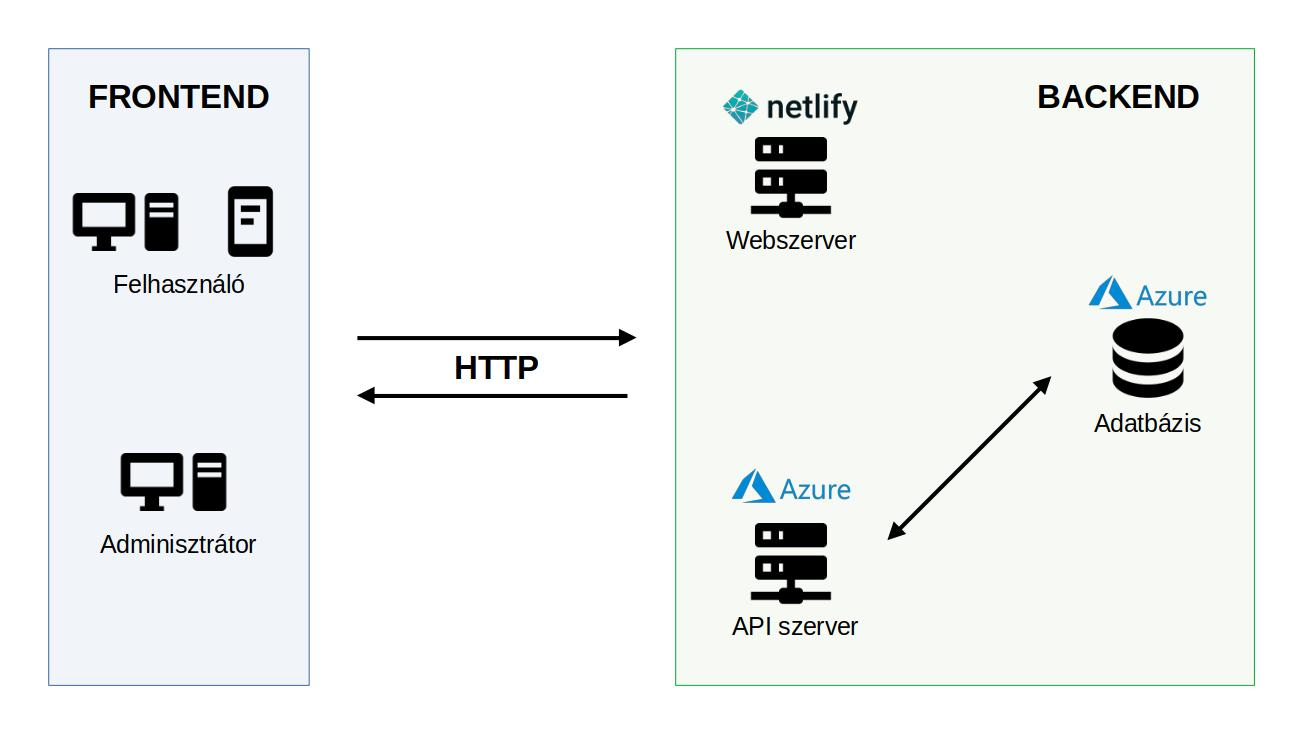
\includegraphics[width=\textwidth]{figures/architecture.jpg}
  \caption{A rendszer architektúrája}
  \label{fig:architecture}
\end{figure}

\section{Frontend}
A frontend a felhasználói felületet biztosítja, amelyen keresztül az emberek interakcióba léphetek a rendszerrel. Jelen esetben a frontend két weboldalból és egy mobilalkalmazásból áll. A két weboldal teljesen elkülönül egymástól, mivel az egyik az adminisztrátoroknak, míg a másik a végfelhasználóknak készült. A weboldalak működése eltér a klasszikustól, mivel ezek egyoldalas alkalmazások (Single Page Application), így kliens oldali renderelést használnak, azaz a felhasználói felületet a kliens oldalon generálja a böngésző, nem pedig a webszerverről érkezik készen. Jelen esetben a webszerver csak a statikus fájlokat szolgáltatja, a dinamikus tartalmakat a kliens oldali JavaScript illeszti be az oldalakba. Ebből a szempontból a weboldal és a mobilalkalmazás működése megegyezik, mivel mindkettő direkt módon az API szerverrel kommunikál, REST kéréseken keresztül. Az adatok JSON típusú szövegként közlekednek a végpontok között az egyszerű feldolgozhatóság végett.

Fontos megemlíteni, hogy egyes API végpontokhoz azonosítás szükséges, ami úgynevezett tokonek segítségével valósul meg. Úgy a weboldalak, mint az alkalmazás eltárolják a szervertől kapott tokenet és hozzáfűzik minden API kéréshez, ezzel azonosítva a felhasználót. Egyes oldalakon térképek is megjelennek, amelyeket a web esetében a MapBox, míg a mobil esetében a Google Maps szolgáltat. Mindkét esetben az adott platformhoz és technológiához közelebb álló térképszolgáltatót választottam, hogy a legjobb felhasználói élményt biztosítsam.

\section{Backend}
A backend a szerveroldali logikát és az adatbázis elérést biztosítja. Ahogyan az előbbiekben említettem, a weboldalak API hívásokon keresztül kapják meg az adatokat és dinamikusan jelenítik meg őket, ezért nincs egy olyan webszerver, amely backend oldalon renderelné ki a weboldalakat, csak egy olyan, amely statikus fájlokat szolgáltat. Ez azt eredményezi, hogy a webszerver nem tartalmaz üzleti logikát és az adatbázissal sincs összeköttetésben.

Ezzel szemben van egy API szerver, amely az összes felhasználói felületet kiszolgálja adatokkal. Az ő feladata az adatbázissal való kommunikáció, az adatok feldolgozása és az ezek elérhetővé tétele a frontend számára, API végpontok formájában. Ez a komponens kezeli a felhasználóktól érkező kéréseket is, amelyek az adatbázist szeretnék módosítani. Minden ellenőrzés, biztonsági vizsgálat is itt folyik le, hogy a frontend csak a megfelelő adatokhoz férhessen hozzá és csak azokat módosíthassa. 

Az adatok kiszolgálásának folyamatában az adatbázisnak csak az a feladata, hogy a felhasználók, buszok, járatok, megállók és jegyek adatait biztonságosan tárolja és azokat az API szerver számára elérhetővé tegye olvasásra és módosításra is.

Részletesebb leírást a backend felépítéséről és működéséről Zsigmond Attila kollégám dolgozatában lehet találni \cite{bus4userver}, mivel ő foglalkozott ezzel a résszel.

\section{Kommunikáció}
A felek közötti kommunikációt szemlélteti a \ref{fig:secvential-navigation} ábrán megjelenített szekvencia diagram, amely az utazás megtervezésének folyamatát írja le. A felhasználó a frontend felületen keresztül kiválasztja az indulási és célállomást, valamint az utazás idejét, majd a rendszer a backend felé elküldi a kiválasztott adatokat. A backend először ellenőrzi a kérést, majd a megfelelő adatokat lekérdezi az adatbázisból és a választ visszaküldi a frontendnek, ahol az megjelenik a felhasználó számára. Amennyiben valahol hiba történik, a rendszer a hiba okát is visszajelzi a felhasználónak.

\begin{figure}[H]
  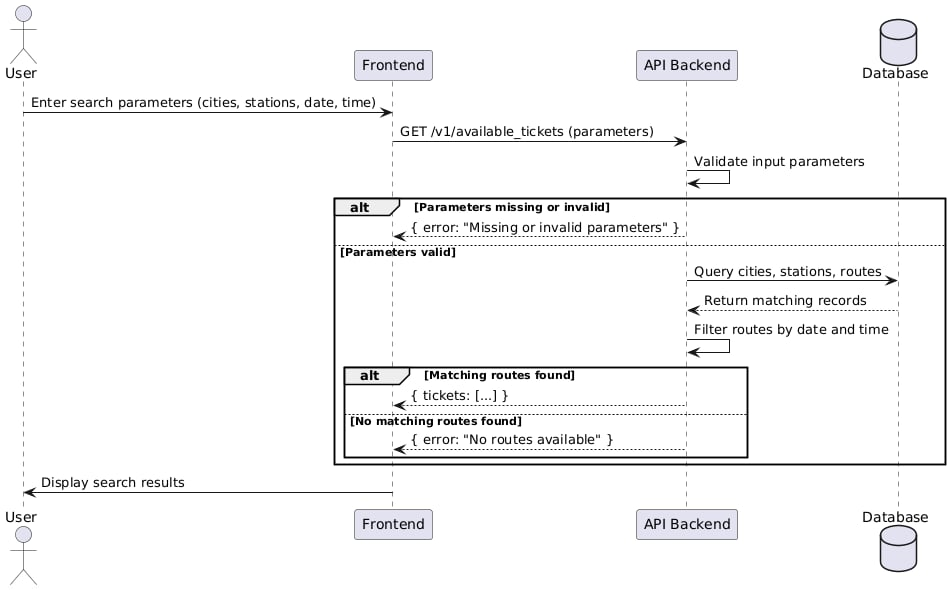
\includegraphics[width=\textwidth]{figures/secvential-navigation.jpeg}
  \caption{Az utazás megtervezésének folyamata}
  \label{fig:secvential-navigation}
\end{figure}

Ugyanígy leírható a jegyvásárlás folyamata is, ahol a felhasználó a frontend felületen keresztül kiválasztja a megfelelő jegyeket, majd a rendszer a backend felé elküldi a kiválasztott adatokat. A backend ellenőrzi a kérést és ha az nem tartalmazza a bejelentkezett felhasználót, akkor visszaküldi a bejelentkezési kérést a frontendnek. Ha a kérés helyes, akkor a szerver létrehozza a jegyet vagy jegyeket az adatbázisban, majd küld egy e-mailt a felhasználónak és a frondendnek is visszaküldi a létrehozott jegyek azonosítóit. Ennek megfelelően a frontend megjeleníti a jegyeket, vagy adott esetben a hibaüzeneteket a felhasználó számára. Az ezt a folyamatot szemléltető szekvencia diagram a \ref{fig:secvential-buy-ticket} ábrán látható.

\begin{figure}[H]
  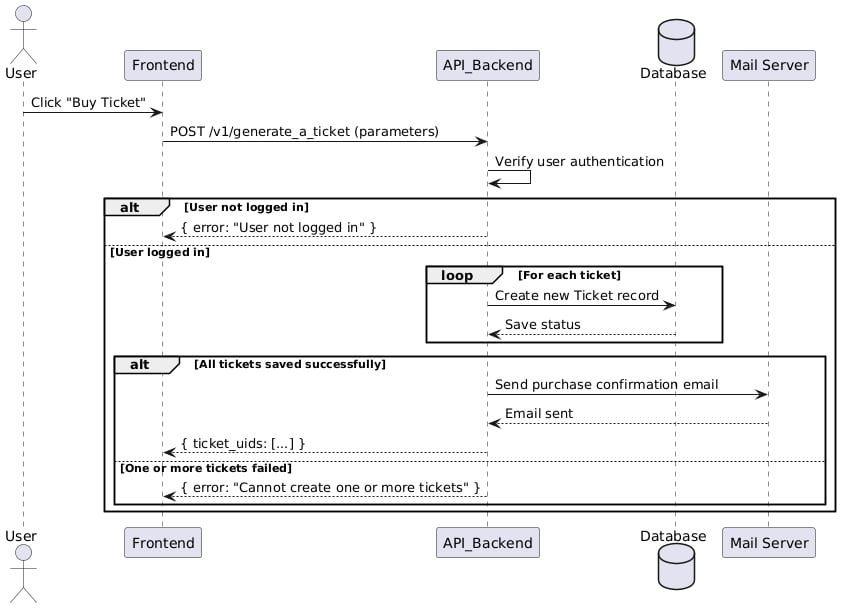
\includegraphics[width=\textwidth]{figures/secvential-buy-ticket.jpeg}
  \caption{A jegyvásárlás folyamata}
  \label{fig:secvential-buy-ticket}
\end{figure}

\section{Felhasznált technológiák}
A felhasználói és az admin weboldalak Vue.js keretrendszerben készültek, Vuetify komponenseket felhasználva. Azért esett a választásom erre a kombinációra, mert a Vue által gyors és hatékony weboldalakat lehet létrehozni, a Vuetify pedig felgyorsítja a fejlesztést előre elkészített, jól kinéző komponensek szolgáltatásával.
A mobil platformokra szánt alkalmazás elkészítéséhez Flutter technológiát használtam, mert ennek segítségével egyetlen kódbázisból ki lehet generálni Android és iOS készülékekre is a natív alkalmazást, amely hatékonyan működik minden eszközön a keretrendszer optimalizációi miatt.
Mindkét implementáció a Material Design irányelveit követi, mert ez egy szép és egységes felületet biztosít a felhasználók számára, bármilyen eszközön használják a Bus4U-t.

\subsection{Vue.js}
A Vue.js egy progresszív JavaScript keretrendszer, amelyet azért hoztak létre, hogy a webes felhasználói felületek fejlesztése egyszerűbb és gyorsabb legyen. A JavaScript keretrendszerek célja, hogy megkönnyítsék a webprogramozást, azáltal hogy előre megírt osztály- és függvénykönyvtárakat szolgáltatnak, amelyek segítenek lerövidíteni a fejlesztési időt. Első ilyen keretrendszer a jQuery volt, amely a DOM (Document Object Model) manipulációt és az AJAX (Asynchronous JavaScript And XML) hívásokat tette egyszerűbbé, majd később a React és az Angular keretrendszerek jöttek, amelyek a komponens alapú fejlesztést tették lehetővé. Ez a fejlődés viszont mind nagyobb és nagyobb kiterjedésű csomagokat eredményezett, ami kissé csökkentette a weboldalak teljesítményét. A Vue.js ezt a problémát próbálja megoldani, azzal hogy egy könnyű, gyors és hatékony keretrendszert kínál, amely egy Virtuális DOM modell segítségével gyorsítja a futást és amelynek a forráskódja akár 24 Kb-ra is zsugorítható, így viszonylag gyors a betöltése is \cite{vueinaction}.

A Vue.js két alapköve a deklaratív UI felépítés és a reaktivitás. A deklaratív felépítés azt jelenti hogy az alap HTML kódot a Vue kiegészíti egy saját sablon-szintaxissal, amely lehetővé teszi a változók beékelődését a HTML kódba. A reaktivitás azt jelenti, hogy amikor a HTML sablonban felhasznált JavaScript változók értéke megváltozik, akkor a Vue érzékeli ezt és automatikusan megváltoztatja a megjelenített HTML kódot, így mindig a legfrissebb adatokat látja a felhasználó. Ugyanez végbemegy fordított irányban is, mert a felhasználói interakciók eredményeképpen a Vue automatikusan frissíti a háttérben lévő változókat is, így lesz a kommunikáció a DOM és a Vue között kétirányú \cite{vueinaction,vue3}.

A Vue keretrendszer egyik legnagyobb előnye, hogy könnyen tanulható és alkalmazható, így gyorsan lehet vele fejleszteni. Ennek egyik oka, hogy komponens alapú, amely lehetővé teszi a weboldalak felépítését újrafelhasználható, különálló komponensekből, amelyeket később össze lehet fűzni egy nagyobb alkalmazássá. Ezek úgynevezett Single-File Component-ek (egyfájlos-komponensek) formájában jelennek meg, amely azt jelenti, hogy az adott komponens HTML, CSS és JavaScript kódja mind egy fájlon belül található, ezzel egy átlátható és moduláris alkalmazásfelépítést eredményezve \cite{vue3}. Emellett a Vue nagyon jó online dokumentációval rendelkezik, amelyben minden funkció részletesen le van írva, de különleges problémákkal és kérdésekkel a dinamikusan növekvő fejlesztői közösséghez is lehet fordulni, így mindig könnyen meg lehet találni az éppen szükséges információt és nagyon gyorsan el lehet sajátítani a keretrendszer használatát \cite{vueinaction}.

A Vue legújabb verziója a Vue 3, amely a komponensek leírására 2 féle API-t \footnote{Application Programming Interface} is biztosít: Options és Composition. A Composition API a 3-as verziótól került bevezetésre és különféle teljesítménybeli optimalizációkat tartalmaz a régi Options API-jal szemben, de a szintaxisa is egyszerűbb, mert közelebb áll az alap JavaScript szintaxisához \cite{vue3}. A Vue 3 a TypeScript támogatását is bevezette, amely egy statikus típusellenőrző nyelv a JavaScript fejlesztéséhez és amely segít a hibák korai felfedezésében, valamint a kód minőségének javításában. Én a munkám során a Vue 3-at és a Composition API-t használtam, mivel ezek a legújabb és legelőnyösebb technológiák jelenleg.

Fontos megemlíteni a Vue ökoszisztémájába tartozó egyéb eszközöket is, amelyek segítik a fejlesztést. Ilyen például a Vue Router, amely a weboldalak közötti navigációt teszi lehetővé, a Pinia, amely a globális állapotkezelést segíti, a Vite, amely a projekt generálását és a fejlesztést segíti, vagy a Vitest amely a teszteléshez szolgáltat hasznos eszközöket \cite{vue3}. Ezek közül kiemelném a Vite nevű build tool-t (építő eszközt), amelynek a gyors újratöltés funkciója figyeli a forráskódban létrejött módosításokat és azonnal frissíti a weboldalt, így a fejlesztőnek nem kell manuálisan a frissítés gombot nyomogatni minden begépelt kódsor után.

A felhasználó szemszögéből a leglátványosabb tulajdonság, hogy nagyon gyors a betöltés és a navigáció, mivel a Vue Single Page Application üzemmódja és a Vue Router kombinációja által lényegében csak egyszer töltődik be a webalkalmazás, utána az oldalak közötti navigáció során csak a tartalom frissül, nem pedig az egész oldal, így lényegesen kevesebb adat közlekedik a hálózaton keresztül és a böngészőnek is kevesebb dolga van az oldalak megjelenítésénél \cite{vue3}. Ezeknek a funkcióknak a segítségével egy gyors és hatékony felhasználói felületet lehet készíteni, amely a gyengébb hálózati lefedettséggel és a gyengébb hardverrel rendelkező eszközökön is jól használható.

\subsection{Vuetify}
A Vuetify egy Material Design alapú Vue.js-re épülő, nyílt forráskódú UI könyvtár, amely lehetővé teszi a gyors és egyszerű felhasználói felületek készítését, azáltal hogy rengeteg előre elkészített Vue komponenst tartalmaz, amelyeket egyszerűen be lehet integrálni a weboldalba, így sok időt lehet vele spórolni. A Vuetify segítségével gyorsan és hatékonyan sikerült felépítenem a weboldalak felhasználói felületeit, mi több, ezek jól néznek ki és jól is működnek minden tesztelt eszközön.

\subsection{Flutter}
A Flutter egy nyílt forráskódú, Google által kifejlesztett, cross-platform, UI készítő keretrendszer, amely lényege, hogy egyetlen kódbázisból ki lehet generálni az alkalmazásokat a legnépszerűbb platformokra. Ezek a platformok a következők: Android, iOS, Windows, macOS, Linux, valamint a web.

A Flutter a Dart programozási nyelvet használja, amely szintén a Google fejlesztése. Ez egy modern, típusos, objektum orientált nyelv, amelyet könnyet és gyorsan el lehet sajátítani. Eredetileg a Dart a JavaScript lecserélésére volt létrehozva a webfejlesztésben, ami eddig nem tudott valósulni, viszont idővel a Flutter technológia alapjává vált és így tett szert népszerűségre. A Flutter egyik nagy előnye, hogy egy widget rendszert használ, amely lehetővé teszi a felhasználói felületek egyszerű és gyors elkészítését, valamint a különböző platformokra történő kiadást. Ezek a widgetek alapértelmezetten a Material Designra épülnek, így egy egységes, intuitív és a felhasználót megragadó felület építhető fel belőlük \cite{materialdesign}, amely összhangban van a Vuetify webes komponenseivel is. A Flutter egy másik nagy előnye, hogy a natív alkalmazásokhoz hasonlóan gyors és hatékony, mivel natív kódra fordítja le a Dart kódot, így a lehető legjobb teljesítményt nyújtja, bármilyen platformról is legyen szó \cite{flutterinaction}.

A funkció amely nagyban megkönnyíti a fejlesztést és a tesztelést, az a Hot Reload, amely lehetővé teszi a fejlesztők számára, hogy azonnal láthassák a változtatásokat a kódban, anélkül hogy újra kellene indítani az alkalmazást \cite{flutterinaction}. Ez a Flutter funkció sokáig egyedüli volt a mobilfejlesztésben, az Android és az iOS csak később vezetett be hasonló funkciókat.

A Flutterben való alkotás hatékonyságát tovább növeli az, hogy egy részletes online dokumentációval rendelkezik, és hogy a Pub Package Manager-t (Csomagkezelőt) használja, amely rengeteg előre elkészített csomagot tartalmaz, az egyszerű UI komponensektől kezdve, a komplex háttérfolyamatokig. Ehhez csak meg kell keresni a megfelelőt a \url{pub.dev} weboldalon és be kell illeszteni az alkalmazásba \cite{flutterinaction}.

Jelen projekt esetében, mivel a webes felületet a Vue.js és a Vuetify keretrendszerekkel készítettem, a Flutter használatakor inkább a mobilos platformokra koncentráltam, tehát az Androidra és az iOS-re. Összességében így kijelenthető, hogy a legnépszerűbb platformok le lettek fedve és bárki, bármilyen eszközről el tudja érni a Bus4U-t.

\section{Fejlesztői eszközök}

A fejlesztés során számos eszközt használtam, amelyek segítették a munkámat és a hatékonyságomat. A legfontosabb ezek közül a kódszerkesztő, amelynek a Visual Studio Code-ot használtam, mert ez egy könnyű, gyors és hatékony eszköz, amely támogatja a Vue.js és a Flutter keretrendszereket is. A Visual Studio Code egyik legnagyobb előnye, hogy jól testreszabható a rengeteg letölthető kiegészítő által, amelyek segítségével a fejlesztők szinte bármilyen programozási nyelvet és keretrendszert használhatnak benne\footnote{Visual Studio Code: \url{https://code.visualstudio.com/}}.

Mivel a projekten nem egyedül dolgoztam, hanem egy kollégámmal, így szükség volt egy eszközre amelyben vezetni tudjuk a feladatokat átlátható módon. Erre a Jira-t használtuk, amely egy online projektmenedzsment eszköz, amelynek segítségével könnyen lehet követni a feladatokat, a fejlesztés állapotát és a határidőket is egy kanban board-on.\footnote{A projekt Jira oldala: \url{https://bus4u.atlassian.net/jira}} Itt felbontottuk az egész projektet kisebb feladatokra, úgynevezett taszkokra, amelyekhez kódneveket rendeltünk hozzá. Ezeknek a formája \textit{BUS-XX} volt, ahol az \textit{XX} egy sorszám, amely a feladatok sorrendjét jelöli. A feladatok állapotát a Jira segítségével tudtuk követni, amelyek lehetnek: "To Do", "In Progress" és "Done". A taszkok nevei tartalmazták a feladat rövid leírását, de hozzá lehetett adni bővebb leírást és hozzászólásokat is. Az \ref{fig:jira} ábrán látható a Jira tábla, amelyen a feladatok vannak elhelyezve.

\begin{figure}[H]
  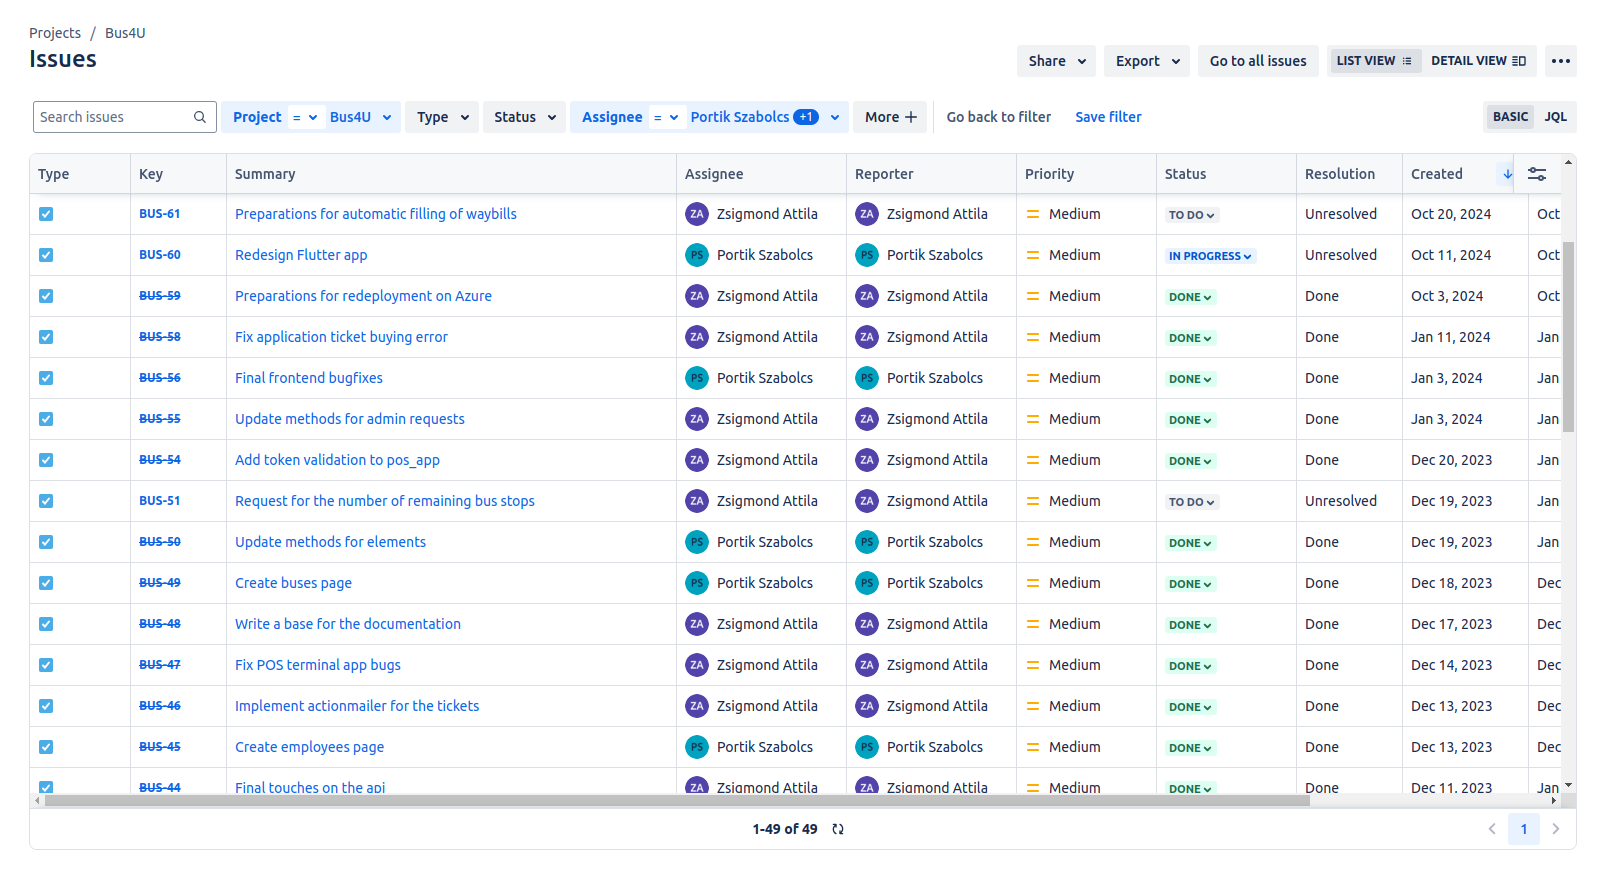
\includegraphics[width=\textwidth]{figures/jira.png}
  \caption{Feladatok a Jira-ban}
  \label{fig:jira}
\end{figure}

Verziókövetésre a Git-et használtuk, GitHub-al kiegészítve, így biztonságosan tudtuk tárolni a kódot és a változtatásokat is könnyen nyomon tudtuk követni. A GitHub abban is segített, hogy összehangoljuk a frontend és a backend fejlesztését a kollégámmal, valamint hogy több, különböző eszközről is tudjunk dolgozni. A munka során branch-ekre (ágakra) osztottuk a projektet, úgy hogy a fő ág mellett volt egy develop nevű ág és ebből váltak ki az egyes feladatok mellékágai, amelyek mind egy-egy Jira taszknak feleltek meg. A mellékágak nevei tartalmazták a taszk kódját, így össze lehetett hangolni a verziókövetést a kanban táblával. A branchek használata megkönnyítette és strukturáltabbá tette a közös munkát. A Git és a branch-ek egyszerűbb kezelésére a GitKraken nevű eszközt használtam, amely egy grafikus felületet biztosít a Git parancsokhoz, így átláthatóbbá válik a rendszer. A GitKraken kezelőfelülete a projekt ágrajzával az \ref{fig:gitkraken} ábrán látható.

\begin{figure}[H]
  
\includegraphics[width=\textwidth]{figures/gitkraken.png}
  \caption{Verziókövetés GitKraken segítségével}
  \label{fig:gitkraken}
\end{figure}

\section{Kitelepítés}
A weboldalak ki lettek telepítve Netlify-ra, hogy könnyebben tesztelhetőek és bemutathatóak legyenek. A Netlify egy olyan szolgáltatás, amely lehetővé teszi a statikus weboldalak gyors és egyszerű kiszolgálását a GitHub repository-ból automatikusan, így a változtatások a \textit{git push} parancs után azonnal megjelennek a weben. A felhasználói weboldal a \url{https://bus4u.netlify.app}, az adminisztrátori weboldal pedig a \url{https://bus4u-admin.netlify.app} címen érhető el.